%%%%%%%%%%%%%%%%%%%%%%%%%%%%%%%%%%%%%%%%%
% Short Sectioned Assignment
% LaTeX Template
% Version 1.0 (5/5/12)
%
% This template has been downloaded from:
% http://www.LaTeXTemplates.com
%
% Original author:
% Frits Wenneker (http://www.howtotex.com)
%
% License:
% CC BY-NC-SA 3.0 (http://creativecommons.org/licenses/by-nc-sa/3.0/)
%
%%%%%%%%%%%%%%%%%%%%%%%%%%%%%%%%%%%%%%%%%

%--------------------------------------------------------------------------------
%	PACKAGES AND OTHER DOCUMENT CONFIGURATIONS
%--------------------------------------------------------------------------------

\documentclass[paper=a4, fontsize=11pt]{scrartcl} % A4 paper and 11pt font size

\usepackage{graphicx}
\usepackage{caption}
\usepackage{subcaption}
\usepackage[T1]{fontenc} % Use 8-bit encoding that has 256 glyphs
\usepackage{fourier} % Use the Adobe Utopia font for the document - comment this line to return to the LaTeX default
\usepackage[english]{babel} % English language/hyphenation
\usepackage{amsmath,amsfonts,amsthm} % Math packages

\usepackage{sectsty} % Allows customizing section commands
\allsectionsfont{\centering \normalfont\scshape} % Make all sections centered, the default font and small caps

\usepackage{fancyhdr} % Custom headers and footers
\pagestyle{fancyplain} % Makes all pages in the document conform to the custom headers and footers
\fancyhead{} % No page header - if you want one, create it in the same way as the footers below
\fancyfoot[L]{} % Empty left footer
\fancyfoot[C]{} % Empty center footer
\fancyfoot[R]{\thepage} % Page numbering for right footer
\renewcommand{\headrulewidth}{0pt} % Remove header underlines
\renewcommand{\footrulewidth}{0pt} % Remove footer underlines
\setlength{\headheight}{13.6pt} % Customize the height of the header

\numberwithin{equation}{section} % Number equations within sections (i.e. 1.1, 1.2, 2.1, 2.2 instead of 1, 2, 3, 4)
\numberwithin{figure}{section} % Number figures within sections (i.e. 1.1, 1.2, 2.1, 2.2 instead of 1, 2, 3, 4)
\numberwithin{table}{section} % Number tables within sections (i.e. 1.1, 1.2, 2.1, 2.2 instead of 1, 2, 3, 4)

\setlength\parindent{0pt} % Removes all indentation from paragraphs - comment this line for an assignment with lots of text

\usepackage[hidelinks]{hyperref}

%----------------------------------------------------------------------------------------
%	TITLE SECTION
%----------------------------------------------------------------------------------------

\newcommand{\horrule}[1]{\rule{\linewidth}{#1}} % Create horizontal rule command with 1 argument of height

\title{
  \normalfont \normalsize
  \textsc{EPFL CS-444 Virtual Reality} \\ [25pt] % Your university, school and/or department name(s)
  \horrule{0.5pt} \\[0.4cm] % Thin top horizontal rule
  \huge Project proposal: 3D File Explorer \\ % The assignment title
  \horrule{2pt} \\[0.5cm] % Thick bottom horizontal rule
}

\author{Florian Junker, Sidney Bovet} % Your name

\date{\normalsize\today} % Today's date or a custom date

\begin{document}

\maketitle % Print the title

%----------------------------------------------------------------------------------------
%	PROBLEM 1
%----------------------------------------------------------------------------------------

\section{General Idea}

In the recent years, many people have released interesting applications and demos for various VR devices such as Oculus, Razer Hydra, Kinect, Leapmotion, and many more. The problem we identified is that most of these applications are either games or closer to a poof of concept than a really useful app for the user. We propose to take two of these devices, namely the Oculus and the Leapmotion sensor, and to produce a useful app that could possibly be used by people for more than five minutes. Our general idea is to create an interactive app-launcher for other Oculus applications so that the user stays during the whole interaction within the virtual environment.

%------------------------------------------------

\section{Work previously done}

The main inspiration for this project comes from a demo made by a VR enthusiast known as HOCgaming. This video is pointed to in section \ref{sec:refs} and shows a user interface inspired by a famous anime. While being extremely interesting and very enthusing, this application suffers from the syndrome expressed above: it is enjoyable for ten minutes and then lacks usefulness.

On the other hand a quite successful project in its usability is mozvr. It is an extension to Mozilla Firefox that enables the user to browse some prepared webpages using an Oculus and possibly other VR devices. It is to us a great example of what a good application can be in terms of usability and usefulness.

One last work we spotted as interesting is an interactive 3D desktop application that enables the user to order a virtual desktop full of files, move them around, stack them and so on. We find this design quite intuitive and close to a real-life organisation (more realism than magic in this case).

%------------------------------------------------

\section{Devices and API}
We want to use the Oculus as the head-tracking system of our project and the Leapmotion sensor as a 3D input device. 

%------------------------------------------------

\section{Detailed idea}


%------------------------------------------------

\section{References}
\label{sec:refs}
\begin{enumerate}
\item Main inspiration: \url{https://www.youtube.com/watch?v=jLp3W1gbhRk&t=51}
\item MOZVR: \url{http://mozvr.com/}
\item BumTop 3D Desktop: \url{https://www.youtube.com/watch?v=M0ODskdEPnQ}
\end{enumerate}


\begin{figure}
\centering
\begin{subfigure}[c]{0.4\textwidth}
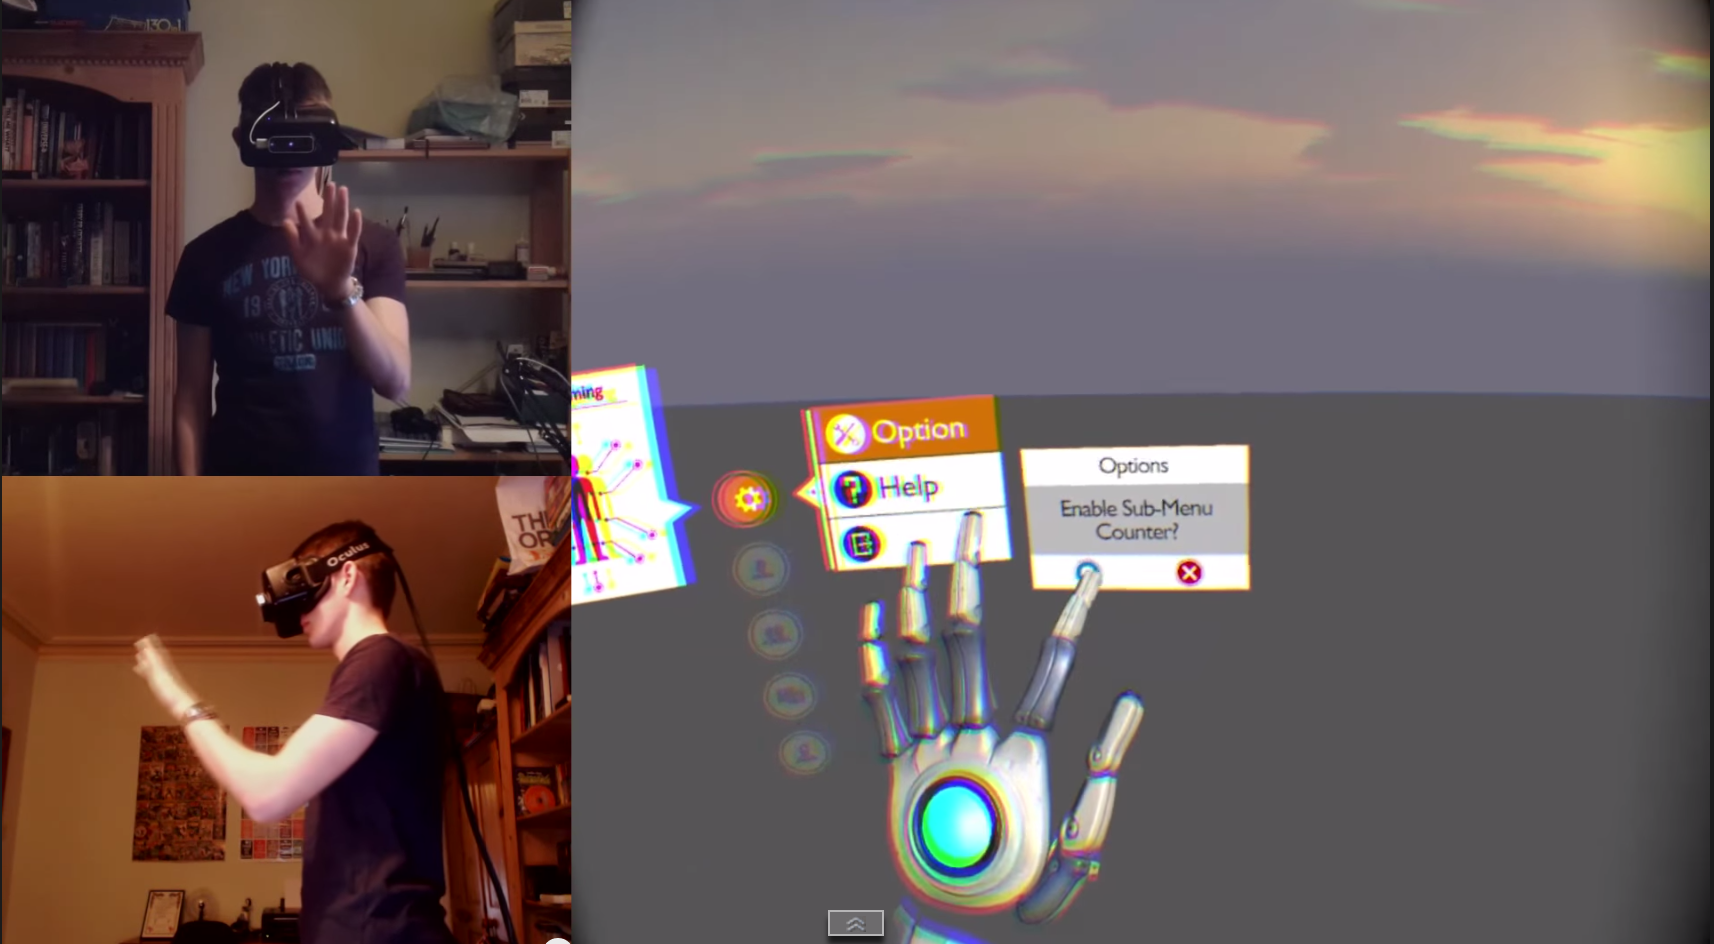
\includegraphics[width=1\textwidth]{sao.png}
\caption{\label{fig:frog}SAO like menu}
\end{subfigure}%
\qquad%
\begin{subfigure}[c]{0.4\textwidth}
\centering
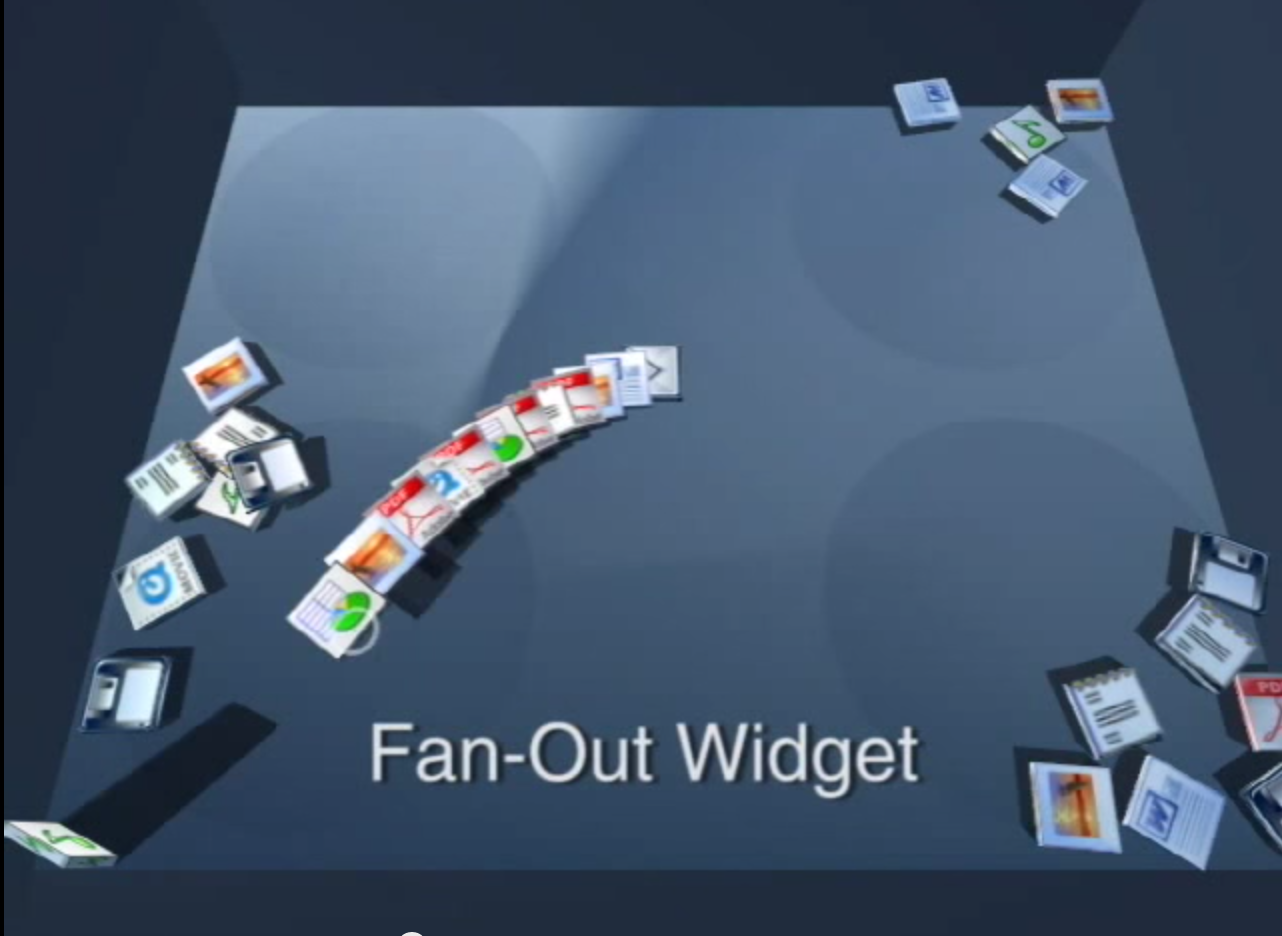
\includegraphics[width=1\textwidth]{fs.png}
\caption{\label{fig:frog}File system example}
\end{subfigure}
\end{figure}



%----------------------------------------------------------------------------------------

\end{document}
